\subsection{The cost of answering repeated policy queries}
\begin{figure*}[t]
\centering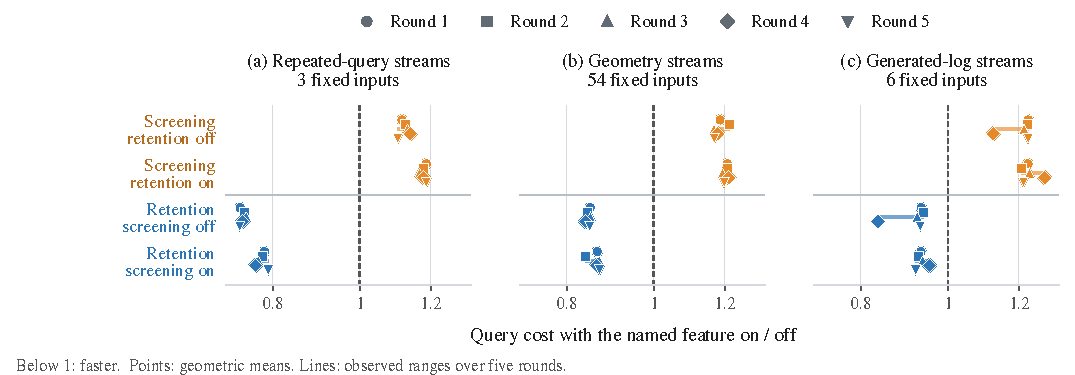
\includegraphics[width=\textwidth]{figures/optimized_v6_compact_factorial.pdf}
\caption{Retention lowers group-average cost; screening does not. Rows toggle the named feature while fixing the other off or on. Each point is one timing round's equal-input geometric mean of on/off cost ratios (R1--R5). Segments span the five rounds, not confidence intervals. The dashed line marks equal cost; below one is faster.}
\label{fig:optimized-factorial}
\end{figure*}
Retention saves the exact group terms that a new query would otherwise recompute; screening first tests whether an exact check can be deferred. All 270,000 responses pass independent exact replay; core plans match evidence,
decisions and native paths. Across the five primary rounds
(Fig.~\ref{fig:optimized-factorial}), retention ratios are
$0.735$--$0.748$ without screening and $0.766$--$0.791$ with it.
Screening ratios are $1.103$--$1.138$ without retention and
$1.165$--$1.186$ with it. Screening also costs more in every geometry and
source-derived group-round mean. Its earlier benefit without retention disappears under optimized arithmetic. Retention reduces cost with either screening setting in all five primary rounds.

The candidate-order control costs $0.833$--$0.882$ times $S_0P_1$ on primary streams,
but is slower in 1/15 primary, 66/270 geometry and 17/30 source-derived
input-round pairs. Retention also has adverse individual cases despite lower
group means. Thus retention lowers group-average cost without guaranteeing an individual speedup. Only this control changes candidate order.
